\documentclass[aima203_lecturenotes_ku.tex]{subfiles}

\setcounter{chapter}{1}
\begin{document}

\chapter{Root Finding}
\section{Introduction}
Roots of an equation
\begin{equation}
  \label{eq:8}
f(x) = 0
\end{equation}
are the zeros, of \(f\), which means, the values of \(x\) that makes the value of \(f\) zero. Basically equations are categorized into two. If \(f\) is a polynomial then the Equation-\ref{eq:8} is a \textbf{polynomial equation} and if \(f\) is a non-polynomial then Equation-\ref{eq:8} is a \textbf{transcendental equation}. For the polynomial equations following results hold:
\begin{enumerate}
\item Every polynomial equation of degree \(n\) has at most \(n\) real roots. These roots may be:
  \begin{enumerate}
  \item Real and distinct
  \item Real and same
  \item Complex
  \end{enumerate}
\item If \(n\) is even and the constant term is negative, then the equation has at-least one positive root and at-least one negative root.
\item The imaginary roots occurs in a pair (conjugate-pair). If the coefficients of \(f\) are rationals then, the irrational roots occurs in pairs (conjugate-pair).
\item Since imaginary roots occurs in a pair, if \(n\) is odd then, the polynomial equation has at least one real root and this root has its sign opposite to that of the last term.

\item \textbf{Descartes' Rule of Signs}
  \begin{enumerate}
  \item[a).] A polynomial equation cannot have more number of positive real roots than the number of changes of signs in the coefficients of \(f(x)\).
  \item[b).] A polynomial equation cannot have more number of negative real roots than the number of changes of signs in the coefficients of \(f(-x)\).
  \end{enumerate}
\end{enumerate}

\section{Characteristic of Numerical Methods}
\begin{enumerate}
\item What do you understand by numerical methods?
\item \textit{Can you name a method that is against numerical method?}
\end{enumerate}

The numerical methods are characterized as follows:
\begin{enumerate}
\item \textbf{Initial guess} \\[1mm]
  It begins with an approximate value of the solution, called as the initial guess.
\item \textbf{Iteration} \\[1mm]
  Then the initial guess is successively corrected by iterations.
\item \textbf{Stopping Criteria} \\[1mm]
  The iterations are done until certain stopping criteria is meet. If we do not specify the stopping criteria then the iterations will run forever. Generally, the stopping criteria is that the solution has reached the required accuracy. The following tests may be used for that purpose.
  \begin{table}[h]
    \centering
    \begin{tabular}{|c|c|r|}
      \hline
      1. &$|x_{i+1} -x_i| \leq E_{\alpha} $ & $E_{\alpha}$ is the absolute error in x. \\[3mm]
      2. &$\displaystyle \frac{|x_{i+1} -x_i|}{x_{i+1}} \leq E_r $ & $E_r$ is the relative error in x. \\[5mm]
      3. &$|f(x_{i+1})| \leq E $ & $E$ is the value of $f$ at root. \\[3mm]
      4. &$|f(x_{i+1})-f(x_i)| \leq E $ \hspace{10mm}& $E$ is the difference in function values. \\[2mm]
      \hline
    \end{tabular}
  \end{table}
\end{enumerate}

\section{Bisection Method}
\begin{mdframed}[style=myframe]
  \begin{theorem}[Bolzano's Theorem]
    \label{Bolzano}
  If f(x) is continuous in \([a,b]\), and if \(f(a)\) and \(f(b)\) are of opposite signs, then \(f(c)=0\) for at least one number \(c \in (a,b)\).
\end{theorem}
\end{mdframed}
The Bisection method is based on Theorem-\ref{Bolzano}. The word ``bisection'' means ``half''. Using this method the root \(c\) of \(f\) is given by \(\displaystyle c \approx \frac{a+b}{2}\). Let \(\displaystyle x_1=\frac{a+b}{2}\). If \(f(x_1) \neq 0\) then, the root, \(c\) lies either in \([a,x_1]\) or in \([x_1,b]\). If \(f(a)f(x_1) <0\) then, \(c\) lies in \([a,x_1]\) else, it lies in \([x_1,b]\). \\[4mm]
At each step of this method, the given interval is bisected, so the length of the interval is halfed. At \(nth\) step the length of the interval is \(\displaystyle \frac{|b-a|}{2^n}\). If the tolerance of the given approximation is \(\epsilon\) then we must have \(\displaystyle \frac{|b-a|}{2^n} \leq \epsilon\). And the number of steps required to reach this accuracy is \(\displaystyle n \geq log_2(|b-a|/\epsilon) = \frac{log_e(|b-a|/\epsilon)}{log_e2}\).

\subsection{Procedure}
\begin{enumerate}
\item Choose two real numbers \(a\) and \(b\) such that \(f(a)f(b) < 0\).
\item Set \(\displaystyle x_0 = 0\) and \(\displaystyle x_1= \frac{a+b}{2}\).
\item Do \\
  \(\displaystyle \epsilon_r = \left | \frac{x_0 -x_1}{x_0} \right |\) \\[1mm]
  If \(\epsilon_r < tolerance\) then \(root = x_1\), \\
  else\\
  \(x_0=x_1\) and if \(f(a)f(x_1) < 0\) then \(\displaystyle x_1= \frac{a+x_1}{2}\) \\
  if \(f(x_1)f(b) < 0\) then \(\displaystyle x_1= \frac{x_1+b}{2}\).
\end{enumerate}

\subsection{Exercise}
Using Bisection Method:
\begin{enumerate}
\item Find a root of \(f(x)=x^3-x-1=0\), correct to \(4\) decimal places.
  \item Obtain a root correct up to three decimal places:
  \begin{multicols}{2}
    a). $x^3-4x-9=0$ \\
    b). $5x\, log_{10}^x -6 = 0$

    \columnbreak

    c). $x^2 +x -cosx = 0$ \\
    d). $x=e^{-x}$
  \end{multicols}
\end{enumerate}

\section{Iteration Method}
Steps:
\begin{enumerate}
\item Re-write the given equation \(f(x)=0\) in the form \(x= \phi (x)\).
  This equation is of \textbf{iterative-type}. Meaning we can substitute a value of \(x\) in \(\phi (x)\) to get another value of \(x\), and continue this process to get the desired value of \(x\), if the iteration is of convergent one.
\item Choose an initial root of \(f\), \(x_0\).
\item \(x_1=\phi (x_0)\), \(x_2= \phi(x_1)\) and so on.
\end{enumerate}
The sequence \(x_0, x_1, x_2, ...\) may not converge to a definite number. But if the sequence converges to a definite number \(\zeta\), then \(\zeta\) is a root of the given equation. The sufficient condition for the sequence of the approximations $x_0, x_1, x_2,...$ by iteration method to converge is that $|\phi ' (x) | < 1$ in some neighborhood (interval) of $x_0$.

\subsection{Exercise}
Using Iteration Method:
\begin{enumerate}
\item Find a root of \(2x-3-cosx=0\), correct to \(3\) decimal places lying in $[3/2, \pi/2]$.
\end{enumerate}

\section{Newton-Rapshon's Method}
Steps:
\begin{enumerate}
\item Choose an initial guess solution of the given equation \(f(x)=0\), \(x_0\).

\item Let \(x_1\) be a solution, which is more close to the exact solution of \(f(x)=0\). Then Using Taylor's expansion of \(f\) about \(x_0\): \[f(x_1)=f(x_0) + (x_1-x_0)f'(x_0) + (x_1-x_0)^2f''(x_0) + ... = 0\]
  Neglecting the second and higher order derivatives, we get
  \begin{equation}
    \label{taylor}
  f(x_0) + (x_1-x_0)f'(x_0)=0
  \end{equation}
  \begin{footnotesize}
    The equation-\ref{taylor} is a linear equation, so this is an linear approximation. This equation is infact the tangent to the curve of the function \(f(x)\) at $(x_0, f(x_0))$. And it is the point $x_1$ where the tangent meets the $x-axis$. So, the next approximation after $x_0$ by Newton-Rapshon's method is the point on $x-axis$, where the tangent to the $f$ at $x_0$ meets the $x-axis$. This point can be solved as follows:
   \end{footnotesize}
  \begin{align*}
    x_1-x_0 & = - \frac{f(x_0)}{f'(x_0)} \\
    x_1 &= x_0 - \frac{f(x_0)}{f'(x_0)}
  \end{align*}

\item Successive approximation are given by \(x_2, x_3, x_4, ...\), where
  \(\displaystyle x_{n+1} = x_n - \frac{f(x_n)}{f'(x_n)}\)
\end{enumerate}

\subsection{Exercise}
Using Newton-Rapshon's Method:
\begin{enumerate}
\item Find a root of \(f(x)=xe^x-1=0\), correct to \(4\) decimal places.
\item Find a non-zero root of the equation $x^2 + 4sinx = 0$ choosing $x_0 = \pi$.
\item Using the Newton-Raphson method, derive a formula for finding the $kth$ root of a positive number $N$ and hence compute the value of $(25)^{1/4}$.

\end{enumerate}

\section{Secant Method}
In Newton-Rapshon's method we use a tangent to the curve to get close to the root of the function. So, Newton-Rapshon's method requires the evaluation of derivatives of the function, which may not always exit. So we replace the tangent, with a secant to approximate the root of the function. \\[2mm]
Steps:
\begin{enumerate}
\item Choose two initial guess solutions of the given equation \(f(x)=0\), \(x_{-1}\) and \(x_0\).

\item The slope of the secant is \(\displaystyle \frac{f(x_0)-f(x_{-1})}{x_0 - x_{-1}}\).

\item  Then equation of the line passing through the points of given by the two initial guesses is \(\displaystyle f(x)-f(x_0)= \frac{f(x_0)-f(x_{-1})}{x_0 - x_{-1}} (x - x_0) \).

\item $x_1$ is the point where the secant meets the $x-axis$ so, $f(x_1)=0$. This gives,
  \begin{align*}
    0-f(x_0) &= \frac{f(x_0)-f(x_{-1})}{x_0 - x_{-1}} (x_1 - x_0) \\
    x_1 -x_0 &= - \frac{x_0 - x_{-1}}{f(x_0)-f(x_{-1})} f(x_0) \\
    x_1 &= x_0 - \frac{x_0 - x_{-1}}{f(x_0)-f(x_{-1})} f(x_0)
  \end{align*}

\item This generalizes to
  \begin{equation}
    \label{eq:secant}
    x_{n+1} = x_n - \frac{x_n - x_{n-1}}{f(x_n)-f(x_{n-1})} f(x_n)
  \end{equation}
\end{enumerate}
You can get this relation-\ref{eq:secant} just by plugging $f'(x_n)=\frac{f(x_n)-f(x_{n-1})}{x_n - x_{n-1}}$ as the slope of the tangent in Newton Rapshon's method is just approximated by the slope of the secant in Secant method.

\subsubsection{Exercise}
\begin{enumerate}
\item Find a real root of the equation $x^3-2x-5=0$ with three iterations.
\end{enumerate}

\section{System of Non-linear equations}
For now we consider only a system of two equations. Let a system of two equations be
\begin{equation}
  \label{system}
  f(x,y)=0, \hspace{1cm} g(x,y)=0
\end{equation}
\subsection{Method of Iteration}
First we assume that the sytem of equations~\ref{system} may be written in the form
\begin{equation}
  \label{iterate}
  x=F(x,y), \hspace{1cm} y=G(x,y)
\end{equation}
where the function $F$ and $G$ satisty the following conditions in a \textbf{closed} neighborhood of $R$ of the root $(\alpha, \beta)$:
\begin{enumerate}
\item[i)] $F$ and $G$ and their firt partial derivatives are continuous in $R$, and
  \item[ii)] $\displaystyle \left | \frac{\partial F}{\partial x} \right | + \left | \frac{\partial F}{\partial y} \right | < 1$ and $\displaystyle \left | \frac{\partial G}{\partial x} \right | + \left | \frac{\partial G}{\partial y} \right | < 1$, for all $(x,y)$ in $R$.
\end{enumerate}
If $(x_0,y_0)$ is an initial approximation to the root $(\alpha, \beta)$, then Equations~\ref{iterate} give the sequence
\begin{equation}
\begin{gathered}
  x_1 = F(x_0,y_0), \hspace{2cm} y_1 = G(x_0,y_0) \\
  x_2 = F(x_1,y_1), \hspace{2cm} y_2 = G(x_1,y_1) \\
  ... \\
  x_{n+1} = F(x_n,y_n), \hspace{2cm} y_{n+1} = G(x_n,y_n)
\end{gathered}
\end{equation}
For faster convergence, recently computed values of $x_i$ may be used in the evaluation of $y_i$ in Equations. Above conditions are sufficient for convergence and in the limit we obtain,
\begin{equation}
  \alpha = F(\alpha, \beta) \hspace{5mm} and \hspace{1cm} \beta=G(\alpha, \beta)
\end{equation}
Hence $(\alpha, \beta)$ is the root of the system~\ref{system}.
\begin{figure}[h]
  \centering
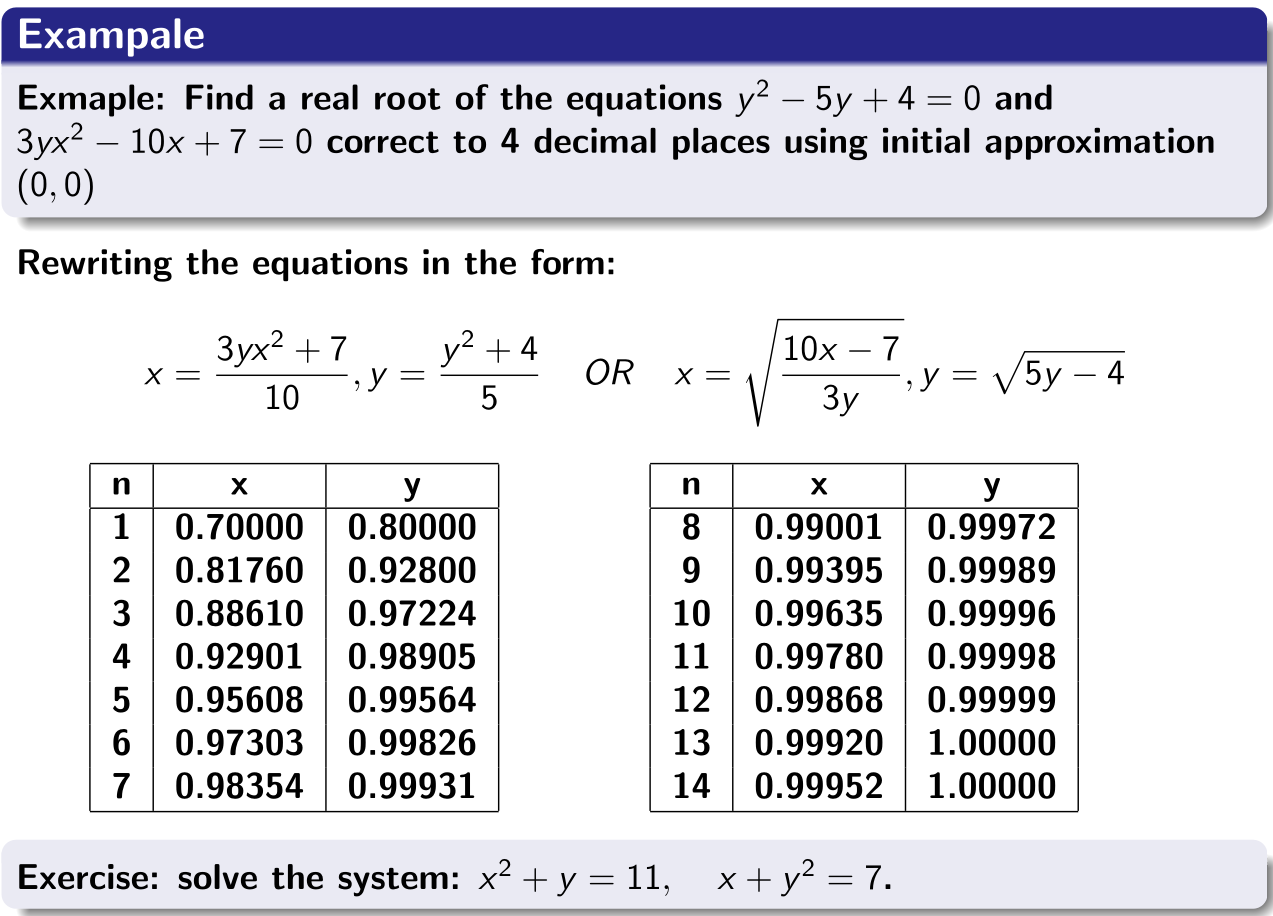
\includegraphics[width=13cm, height=11cm]{secant_example.png}
\end{figure}

\subsection{Newton-Raphson Method}
Let $(x_0,y_0$ be an initial approximation to the root of the system of equations in two variables~\ref{system}. If $(x_0+h, y_0+k$ is the root of the system, then we must have
\begin{equation*}
  f(x_0+h,y_0+k) = 0 \hspace{1cm} g(x_0+h,y_0+k) = 0
\end{equation*}
Assuming that $f$ and $g$ are sufficiently differentiable, we expand both of these functions by Taylor's series to obtain
\begin{equation*}
  \begin{gathered}[t]
    f_0 +h\frac{\partial f}{\partial x_0} + k\frac{\partial f}{\partial y_0}... = 0 \\
    g_0 +h\frac{\partial g}{\partial x_0} + k\frac{\partial g}{\partial y_0}... = 0
  \end{gathered}
\end{equation*}
where, \hspace{5mm} $\displaystyle \frac{\partial f}{\partial x_0} = \left [\frac{\partial f}{\partial x} \right ] _{x=x_0}$, $f_0 = f(x_0,y_0)$, etc \\[1mm]
Neglating the second and higher-order derivatives terms, we get,
\begin{equation}
  \label{taylor}
  \begin{gathered}[b]
    h\frac{\partial f}{\partial x_0} + k\frac{\partial f}{\partial y_0}... = -f_0 \\
     h\frac{\partial g}{\partial x_0} + k\frac{\partial g}{\partial y_0}... = g_0
  \end{gathered}
\end{equation}
The system of equations~\ref{taylor} possesses a unique solution if
$$ D =
\left \vert \begin{matrix}
  \frac{\partial f}{\partial x_0}  & \frac{\partial f}{\partial y_0} \\[2mm]
  \frac{\partial g}{\partial x_0}  & \frac{\partial g}{\partial y_0}
\end{matrix} \right \vert  \neq 0
$$
By Cramer's rule
\begin{equation}
  h= \frac{1}{D}\, \left \vert \begin{matrix}
  -f_0  & \frac{\partial f}{\partial y_0} \\[2mm]
  -g_0  & \frac{\partial g}{\partial y_0}
\end{matrix} \right \vert \hspace{5mm} and \hspace{5mm} k= \frac{1}{D}\, \left \vert \begin{matrix}
  \frac{\partial f}{\partial y_0} & -f_0  \\[2mm]
 \frac{\partial g}{\partial y_0} &  -g_0
\end{matrix} \right \vert
\end{equation}
The new approximations are, therefore
\begin{equation}
  x_1 = x_0 +h \hspace{5mm} and \hspace{5mm} y_1 = y_0 + k
\end{equation}
\begin{figure}[h]
  \centering
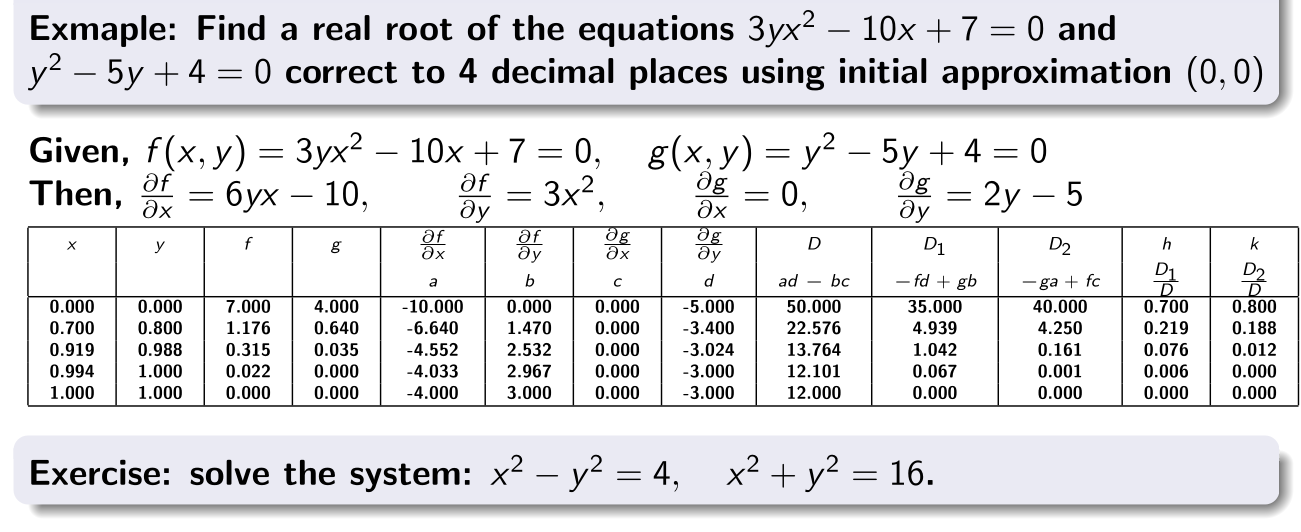
\includegraphics[width=15cm, height=7cm]{newton_example.png}
\end{figure}


\subsection{Exercise}
\begin{enumerate}
\item Find a real root of the system: $y^2-5y+4=0$ and $3x^2y-10x+7 = 0$ correct to $4$ decimal places using initial approximation $(0,0)$.

\item Solve the system: $x^2+y = 11$, $x+y^2 = 7$.

\item Solve the system: $x^2-y^2 = 4$, $x^2+y^2=16$.
\end{enumerate}

\section{Rate of Convergence}
If a sequence $x_1, x_2, x_3, ...$ converges to a value $\alpha$ then, the rate of convergence of the sequence $(x_n)$ to $\alpha$ is $p$, if $p$ is the \textbf{largest} possible number such that:
\begin{equation}
  \label{rateofconverge}
 \lim_{n \to \infty} \;  \frac{|x_{n+1} - \alpha|}{|x_n-\alpha|^p} = constant
\end{equation}
In another words, if $\epsilon _n = x_n-\alpha$ is the error at $nth$ step then, the sequence of the error $(\epsilon_n)$ is a decreasing sequence and the positive integer $p$ defines the rate at which the sequence of error is decreasing and converging to the correct value $\alpha$. So we have,
 e\begin{equation*}
 \lim_{n \to \infty} \;  \frac{|\epsilon _{n+1}|}{|\epsilon _n|^p} = constant
\end{equation*}
When $p=1$, we say the sequence or the method converges \textbf{linearly}, when $p=2$ we say the method converges \textbf{quadratically}, when $1 < p < 2$, we say the method converges \textbf{superlinearly}.

\section{Exercise}
\begin{enumerate}
\item Find the rate of convergence of Bisection Method.
\item The rate of convergence of Newton Rapshon's method is quadratic. Does it converge faster than Bisection Method?
\item Write the rate of convergence of secant method.
\end{enumerate}

\section{Lab Work}
\begin{enumerate}
\item Try a suitable data structure for storing the sequence of outputs in a iteration.
\item Find a way of representing a function.
\item Find an efficient way of evaluating a function or a polynomial.
\item Draw a flow chart for the working of Bisection Method.
\item Writing a function in Python.
\end{enumerate}

\begin{lstlisting}
  def bisection_method(f, a, b, tol=1e-6, max_iter=100):
    """
    Find a root of a function f(x) in the interval [a, b] using the bisection method.

    Parameters:
    f (function): The function for which to find a root.
    a (float): Left endpoint of the interval.
    b (float): Right endpoint of the interval.
    tol (float): Tolerance (stopping criterion).
    max_iter (int): Maximum number of iterations.

    Returns:
    float: Approximation of the root.
    int: Number of iterations performed.
    """
    # Check if the interval contains a root
    if f(a) * f(b) >= 0:
    raise ValueError("Function must have opposite signs at the
    endpoints of the interval.")

    iter_count = 0
    c = a

    while (b - a) / 2 > tol and iter_count < max_iter:
        c = (a + b) / 2  # Midpoint

        if f(c) == 0:
            break  # Exact solution found
        elif f(a) * f(c) < 0:
            b = c  # Root is in left half
        else:
            a = c  # Root is in right half

        iter_count += 1

        return c, iter_count

# Example usage:
if __name__ == "__main__":
    # Define the function whose root we want to find
    def f(x):
        return x**3 - 2*x - 5

    # Initial interval
    a, b = 2, 3

    # Apply bisection method
    root, iterations = bisection_method(f, a, b)

    print(f"Approximate root: {root:.6f}")
    print(f"Found in {iterations} iterations")
    print(f"f(root) = {f(root):.6f}")
\end{lstlisting}

\end{document}





%%% Local Variables:
%%% mode: latex
%%% TeX-master: t
%%% End:
